%___________________________________________________________________________________________________
\chapter{Operations with vectors and matrices} 


\vspace{-.7cm}
\section{Introduction}

This chapter covers two independent topics through examples. In the first place, some essential 
operations of matrix arithmetic are introduced, an operation like the product of two matrices becomes 
extremely simple in programming languages oriented to vector programming. 
In the second place, the concepts of static and dynamic 
data objects are covered. Notice that all the examples are written according to a 
declarative programming, consider reproducing the same results with an imperative programming to 
compare.
    
    \vspace{-.3cm}
    \subsection*{Matrix arithmetic}
    \vspace{-.2cm}

In the context of scientific programming some features like a syntax close to mathematics or
functional oriented programming are desirable for a programming language. In addition, 
array programming is an essential characteristic. It makes
reference to the possibility of operating a whole group of values at the same time, hence, 
the operations applied to a number can also be applied to vectors, matrices and higher dimension arrays
in a easy to write (near to maths) expression greatly simplifying maths computations.
 
Languages like Fortran, MATLAB, R or the NumPy extension of Python support array programming.
Matrix arithmetic are built-in in these languages and expressing the mathematical language in a natural way is feasible.

Take note of the difference between array programming and array processors. The first makes reference to how the programmer 
codes the mathematical operations in its program (a big advantage is obtained from this feature for Scientific Computing as mentioned before). 
The second feature is related to how the processor operates that group of numbers, by performing
all the operations together under the same instruction given to the processor in a considerably increase of speed.
Both features suppose an increase of performance for the coding and executing of scientific programs, however, this chapter is 
oriented to the aspects of the first feature mentioned. 

It is relatively new the development of array programming languages being Fortran the first one to include it in the 90's with the 
ISO/IEC standard 1539:1991. 

The following concepts regarding arrays constructions and operations are covered:

\begin{enumerate} 
    \item Type, rank and dimension of arrays.
    \item Constructors to initialize an array. 
    \item Sectors or slices of arrays. 
    \item Operations among array. 
    
    \begin{enumerate}
        \item Addition. 
        \item Dot product.
        \item Matrix multiplications. 
        \item Hadamard product. 
    \end{enumerate}  
    
\end{enumerate} 

    \vspace{-.5cm}
    \subsection*{Static/Dynamic data objects}

Each data object declared in a program (variables, constants, pointers, arrays, etc.) are either static or dynamic 
which means that the memory storage to hold that piece of data is reserved during compilation time or 
during the execution of the program respectively. Consider the variable \texttt{real :: A(N, N)} declared at the 
beginning of a code, its memory storage is reserved when the program is compiled and this space is not liberated 
until the program has finished the execution. 

Another option to declare and manage the memory storage of a object involves using dynamic allocation. For this case, the 
storage of a variable is not reserved until the program orders it (during execution) and can be changed or freed at any moment. 
This is done through a code like \texttt{real, allocatable :: Ak(:, :, :)}.





%___________________________________________________________________________________________________
\newpage 
\section{Static size vectors and matrices} 

For the following example some basic matrix arithmetic is performed with static data objects. 
Since the sizes of the arrays are known at compile-time, the memory storage can be declared statically. 
The main properties of a static allocation are:

\begin{enumerate}
    \item The memory address and the size are assigned during the compilation of the code in the executable image of your program.
    \item These address and size can not be changed during execution.
    \item Once the program finishes the execution the space is freed.
    \item It is a simple and quick allocation process.
\end{enumerate}


Consider the vectors $V, W \in \mathbb{R}^N$ and the matrices  $ A, B \in { \cal{M}}_{N \times N} (\mathbb{R})$ defined in the following way: 

$$
V = \left[ v_i =\frac{1}{i^2}, \ \ i = 1 \ldots  N \right],
$$

$$
W = \left[ w_i = \frac{(-1)^{i+1}}{2i+1}, \ \ i = 1 \ldots  N \right].
$$

$$
A = \left[ a_{ij} = \left( \frac{i}{N} \right)^{j-1}, \ \ i = 1 \ldots  N, \ \ j = 1 \ldots  N \right].
$$

$$
B = A^T
$$






Some basic notions are summarized now: 

\begin{itemize}
    \item An array is properly declared when it has type, rank and dimension (or extent). 
    All this information comes from the mathematical definition of the vectors and matrices.
    
    \begin{enumerate}
        \item The data type in this case is \texttt{real} since the examples are built with real vectors/matrices. 
        \item Rank is the number of dimensions in the array; a rank-one array represents a column vector (\texttt{V} or \texttt{W}), a rank-two array represents a matrix organised into columns and rows (\texttt{A} or \texttt{B}), etc. 
        \item The extent of each particular dimension is its length, which means, the number of elements in that dimension. All dimensions involved in these examples are equal to \texttt{N}. The bounds of a dimension does not have to start with index \texttt{1}, later some examples with different bounds are shown. 
    \end{enumerate}

    \item Once declared, the initialization of the arrays is performed with constructors. In the case of Fortran the constructors are only used for rank-one arrays so functions like \texttt{reshape} are needed for higher ranks. Three ways are normally used to manually construct an array:
    
    \begin{enumerate}
        \item By a list of values: \texttt{ [ list ] } where 'list' is full of values separated by commas (of the same type declared for the array). 
        For example: 
        
        \texttt{V = [ 3.4, 5.2, 4.5, 2.1 ]} is a column vector of dimension 4 with those values in each position.
        \item An array expression can also be used in the initialization: 
        
        \texttt{V = [ B(2, 3:5) ]} stores in \texttt{V} the list of values in the second row of \texttt{B} from columns \texttt{3} to \texttt{5}.
        \item Using an implicit loop so a list of elements is computed from a loop controlled by a DO variable. Lots of examples of this are used throughout this book: \texttt{V = [ ( 1./i**2, i=1, N ) ]}.
    \end{enumerate}

    \item The sectors of an array are already introduced in this text. Notice that the initialization of \texttt{V} in this example: \texttt{V = [ B(2, 3:5) ]} use a sector of the whole array \texttt{B}. This can also be extended to a whole dimension of an array, i.e. the column 5 of an array \texttt{C} is referred like \texttt{C(:,5)}. Furthermore, alternate values can be selected by specifying a lower and upper bound and the jump between values (see matrix B of Figure \ref{fig:arrays}): \texttt{B(-2:4:2,:)} being the second value \texttt{2} the jump between rows.
    
    \begin{figure}
        \begin{subfigure}[h]{0.5\textwidth}

            \centering
            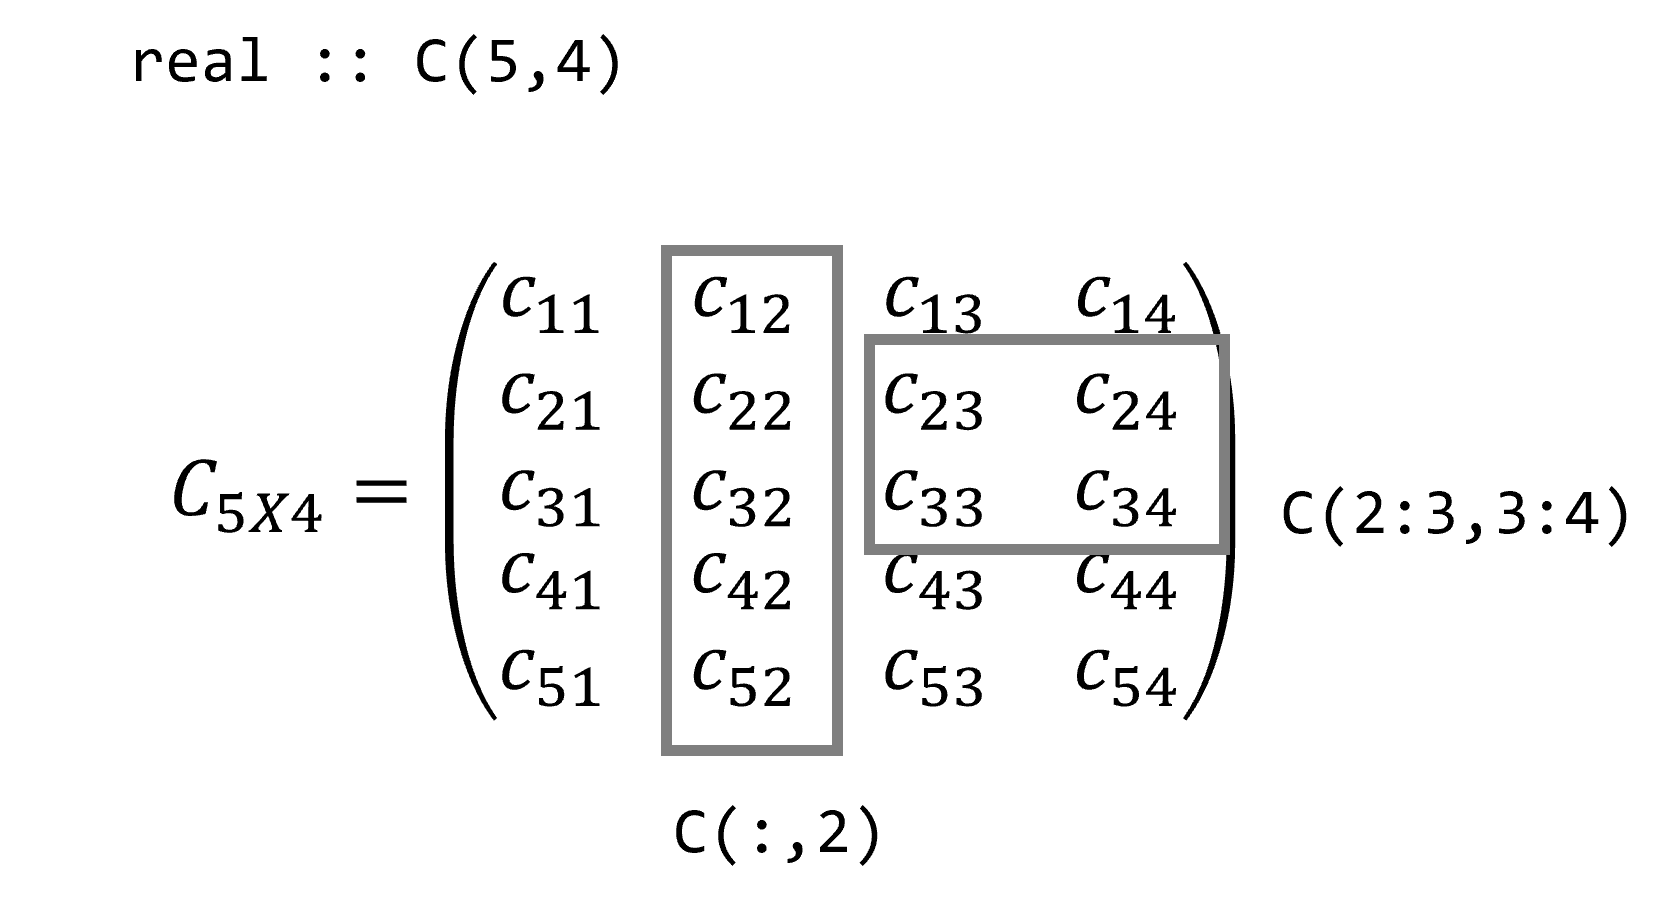
\includegraphics[width = \textwidth]{./doc/Figures/Array1.png}  \\
            \begin{flushleft}
                Rank = 2 \\
                %Extent = 5 and 4 \\
                Size = 20 \\
                Bounds = (1:5, 1:4) \\
                Shape = (5, 4)
            \end{flushleft}

        \end{subfigure}
        \hspace{\fill}
        \begin{subfigure}[h]{0.5\textwidth}

            \centering
            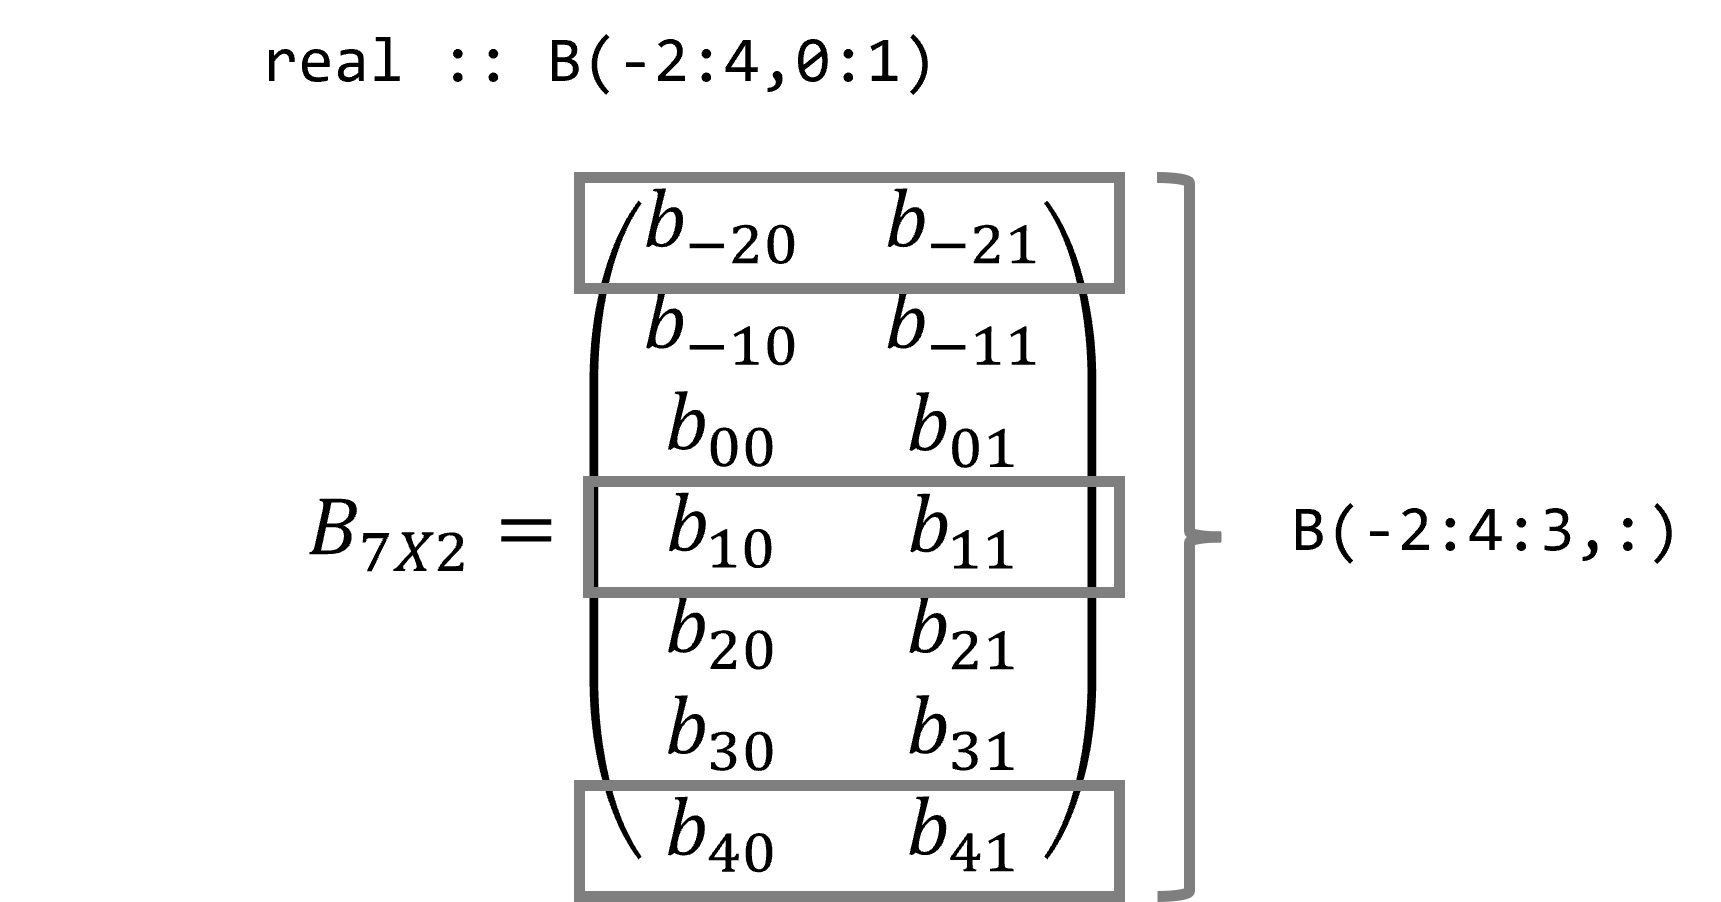
\includegraphics[width = \textwidth]{./doc/Figures/Array3.png}  \\
            \begin{flushleft}
                   Rank = 2 \\
                   %Extent = 7 and 2 \\
                   Size = 14 \\
                   Bounds = (-2:4, 0:1) \\
                   Shape = (7, 2)
            \end{flushleft}

        \end{subfigure}
        \caption{Properties of a couple of arrays.}   \label{fig:arrays}
    \end{figure}
    
    \item Some operations to be used with real matrices are introduced now. Notice that these examples are limited to numeric arrays, reals or even integers, but arrays can be constructed with a different data type. Furthermore, different operations could be created for new data types also created by the programmer. 
    
    Consult the specifications of the following matrix operations to become familiarized with the purpose, inputs and optional arguments allowed.
    As a quick reference: use \texttt{sum} to add all elements of an array, whether it is across one dimension, all the dimensions 
    or only those elements that accomplish with some condition (e.g. $ V_i > 0 $). Use \texttt{dot\_product} to calculate the scalar 
    product of two vectors, \texttt{matmul} for a matrix multiplication and \texttt{transpose} to calculate the transpose of a matrix or vector. 
    In addition, \texttt{maxval} and \texttt{maxloc} return the maximum value of all the elements of an array and its position, whether 
    it is across one specific dimension, the whole array or only for those values that accomplish with a specified condition.
    
    It is mandatory that rank and dimension of the arguments of these intrinsic functions must agree with the mathematical definitions of
    the operations, consider for example how the scalar product of the vector V with a column of A is calculated. The colon symbol : is used
    as an implicit loop for all the elements of column \texttt{N} in the matrix. 
    
\end{itemize}



%\texttt{ (/ list /) } is not used as constructor.


\renewcommand{\home}{./Fortran/sources/Foundations/Algebra} 
\listings{\home/Matrix_operations.f90}{subroutine Matrix_operation_examples}
      {end subroutine}{Matrix_operations.f90}








Take some interesting notes of the previous example. First of all, N is declared as a named constant thanks to the 
\texttt{parameter} attribute. Then, its value is fixed once for all the execution and a try to change it will 
end in a compilation error. Its value is automatically used to declare the 
size of the vectors and matrices involved in the example. 

Secondly, to initialize both V and W the mathematical definition of each component is written by means of an implicit loop (declared with parentheses). 
Two implicit loops are used in the definition of the matrix \texttt{A}, the nested loop \texttt{i} 
calculates the rows while \texttt{j} jumps from one column to the next one. Both loops define 
a $ N * N $ rank-one vector that needs to be reshaped to a ${ \cal{M}}_{N \times N} $ matrix. The function \texttt{reshape} organizes
the components of the vector into columns. 
 
Thirdly, take into account the difference between these operations and the element wise operations that can performed with 
vectors and matrices. Some operations like the addition of two matrices are performed by adding the corresponding elements of both, also, 
many elemental operations on numbers can also be applied to matrices, so the result is an equal shaped array 
with the results of applying the operation to each element. Test the following expressions for matrix addition, Hadamard product (multiplying the corresponding elements of both matrices), cosine or square root of all elements of \texttt{A}:

\begin{verbatim} 
A + B
A*B
cos( A )
SQRT( A )
\end{verbatim}

Finally, take a look at the way the matrix \texttt{B} is written in the screen, by using two loops each row of the matrix is represented element by element.
Compare this way with the simple output of the line \texttt{write(*,*) B} where all the elements are represented by columns and not by rows. This is due to the fact 
that programs store multidimensional arrays in a linear storage and Fortran is a column-major order language where the consecutive elements of a column reside next to each other.





 \newpage 
 \subsection*{Python code}
The whole function can be written in the same manner and almost identically with Python, 
notice from the following example how all vectors and matrices are constructed by using implicit loops. 
Furthermore, the same intrinsic functions are implemented making natural the use of mathematical notation when programming 
(just consider some particularities like indentation or implicit typing). 
\vspace{0.5cm} 
\renewcommand{\home}{./Python/sources/Foundations/Algebra} 
\listings{\home/Matrix_operations.py}{def Matrix_operation_examples}
      {WARNING}{Matrix_operations.py} 










%_______________________________________________________________________________________________
\newpage  
\section{Dynamic allocation of vectors and matrices} 

Consider now that the size of the matrix involved in your code is not known at compile-time, maybe it 
comes from an user input, an external file or it is the result of a previous operation. In this case, dynamic data objects are used 
so the memory storage (address, size, etc.) for the object is allocated or modified during the execution of the program.
The essential statements to manage the memory for this data objects are \texttt{allocate} and \texttt{deallocate} 
while the attribute for the data object is \texttt{allocatable}. The main properties of dynamic data objects are:

\begin{enumerate}
    \item The program decides how much memory reserve for a data objects so it can accommodate any size with no need of re-compiling the code.
    \item Modifications for the memory size are allowed. 
    \item It becomes the programmer responsibility to liberate the memory reserved for non-used arrays in order not to run out-of-memory.
    \item It is generally slower than static allocation. 
\end{enumerate}




Given the square Vandermonde matrix  of $ M \times M $:

$$
A_M =  \left[ a_{ M_{ij} } = \left( \frac{i}{M} \right)^{j-1}, \ \ i = 0, \ldots M-1, \ \  j=0, \ldots M-1 \right],  
$$

determine the following operations:
$$ 
    S = \sum_{M=1} ^{10} \Tr(A_M),  \quad
    S = \sum_{M=1} ^{5} \Tr(A_M^2), \quad
    S = \Tr \left( \sum_{k=0} ^{5} A_M^k  \right),  \quad  M=8 
$$

The following examples are supported by the functions: \texttt{Vandermonde( M )} matrix of a given dimension \texttt{M}, \texttt{trace( A )} trace of a matrix and the recursive function \texttt{power( a, k )} to obtain the kth power of a matrix. Once each function is coded, general operations like these proposed here are easy to implement, remember that each abstraction can now be used in any program where this algebra is needed from now on. 

\newpage 
\renewcommand{\home}{./Fortran/sources/Foundations/Algebra} 
\listings{\home/Dynamic_allocation.f90}{subroutine Matrices_allocation}
{end subroutine}{Dynamic_allocation.f90}


Let's take a deeper look into the program. First of all, notice that the 3-rank object \texttt{Ak} is declared with the attribute \texttt{allocatable} and colons \texttt{:} instead of the dimension specifications. Later, when the dimensions are known, the \texttt{allocate} function is used to reserve the appropriate memory for the variable.

The expression \texttt{trace( Vandermonde(M) )} is coded inside an implicit loop from 1 to 10. This results are constructed in a vector with squared brackets and \texttt{sum} performs the summation of the components of that vector. The mathematical abstraction summation is already implemented in many programming languages. 

The use of many variables is avoided here thanks to a declarative programming. In an imperative programming the Vandermonde matrix would have been stored in a variable \texttt{AM(M,M)}, its trace in a real vector variable used as an input for \texttt{sum}. Do not think that these objects are not used now, the compiler needs them exactly the same in order to operate, however, it automatically reserves memory, stores the intermediate results, returns only the single result needed \texttt{S} and, when the calculation is finished, frees all that temporary memory used in an efficient way. 

The second operation is similar with the exception that now the trace is calculated on the product of two matrices. Fortran, like any common scientific language already has implemented the product between two matrices of reals. As it has been mentioned before, the vector/array programming does not only have advantages in the coding of algebra computing, it has also a better performance when calculating those multiple operations when vector processors are used, so the same operation among a bunch of numbers is performed efficiently. 

For the third operation the variable \texttt{Ak} is dynamically allocated. This 3-rank array is used to store each power of the Vandermonde matrix with bounds 0 to 5 in the third dimension. While normally the indices of any vector or matrix start in 1, is decision of the programmer to modify it so the index automatically responds to a mathematical sense, in this case writing \textit{Ak(:,:,3)} is a reference to the third power, with no need of remembering in which index starts and how many powers are we calculating. If the needed powers of Vandermonde would only have been 4, 5 and 6, we could have allocated the matrix like: \texttt{allocate( Ak(8, 8, 4:6) )}. 

Take note of the full array assignation performed inside the explicit loop. Once the matrix \texttt{Ak} is properly allocated, writing \texttt{Ak(:,:,k) = } is enough to store the result of the kth power of Vandermonde matrix since it is known that the result is an $ 8\times 8 $ matrix. 

%Also, it is mandatory to specify to the function \texttt{sum} that the summation is only performed in the third dimension of \texttt{Ak} so it is adding one matrix to the next one. 


\listings{\home/Dynamic_allocation.f90}{function trace}
{end function}{Dynamic_allocation.f90}

\listings{\home/Dynamic_allocation.f90}{function power}
{end function}{Dynamic_allocation.f90}

For the functions \texttt{power( A, k )} and \texttt{trace( A )} two concepts should be extracted. Firstly, both must be used with square matrices, where both mathematical operations are defined. Secondly, the concept of recursion is used to calculate the kth power of a matrix. Essentially, the kth power of a matrix is the multiplication of that matrix with his $ k-1 $ power. A \texttt{recursive} statement is used for the function declaration so the compiler knows that this function can call to itself in order to calculate smaller instances of its main functionality, which means, it is going to call itself to calculate the $ (k-1) $ power once it tries to compute the kth power and so on until the power needed is 0 so the result is the identity matrix. 



    \subsection*{Python code}
\renewcommand{\home}{./Python/sources/Foundations/Algebra} 
\listings{\home/Dynamic_allocation.py}{def Matrices_allocation}
{return}{Dynamic_allocation.py}


\renewcommand{\home}{./Python/sources/Foundations/Algebra} 
\listings{\home/Dynamic_allocation.py}{def power}
{matmul}{Dynamic_allocation.py}





\section{Memories: Static, Heap, Stack}

It is clear that during the execution of the program certain amount of memory is needed. Data objects or the source code 
must be stored somewhere. The compiler, the linker and the operating system of the machine decides where each piece of data is stored. 
Three regions of the memory can be distinguished for a program (see Figure \ref{fig:Memories}): 
static, heap and stack, each one related to one type of allocation. Notice that the last two memories are dynamic in nature.

Static and dynamic allocation have been already treated. A third way to allocate memory size for data objects is used: 
stack (or automatic) allocation. The compiler is constantly using it 
in order to store temporary arrays used 
inside subroutines/functions or needed for array expressions.


\begin{figure}[h]
    \centering
    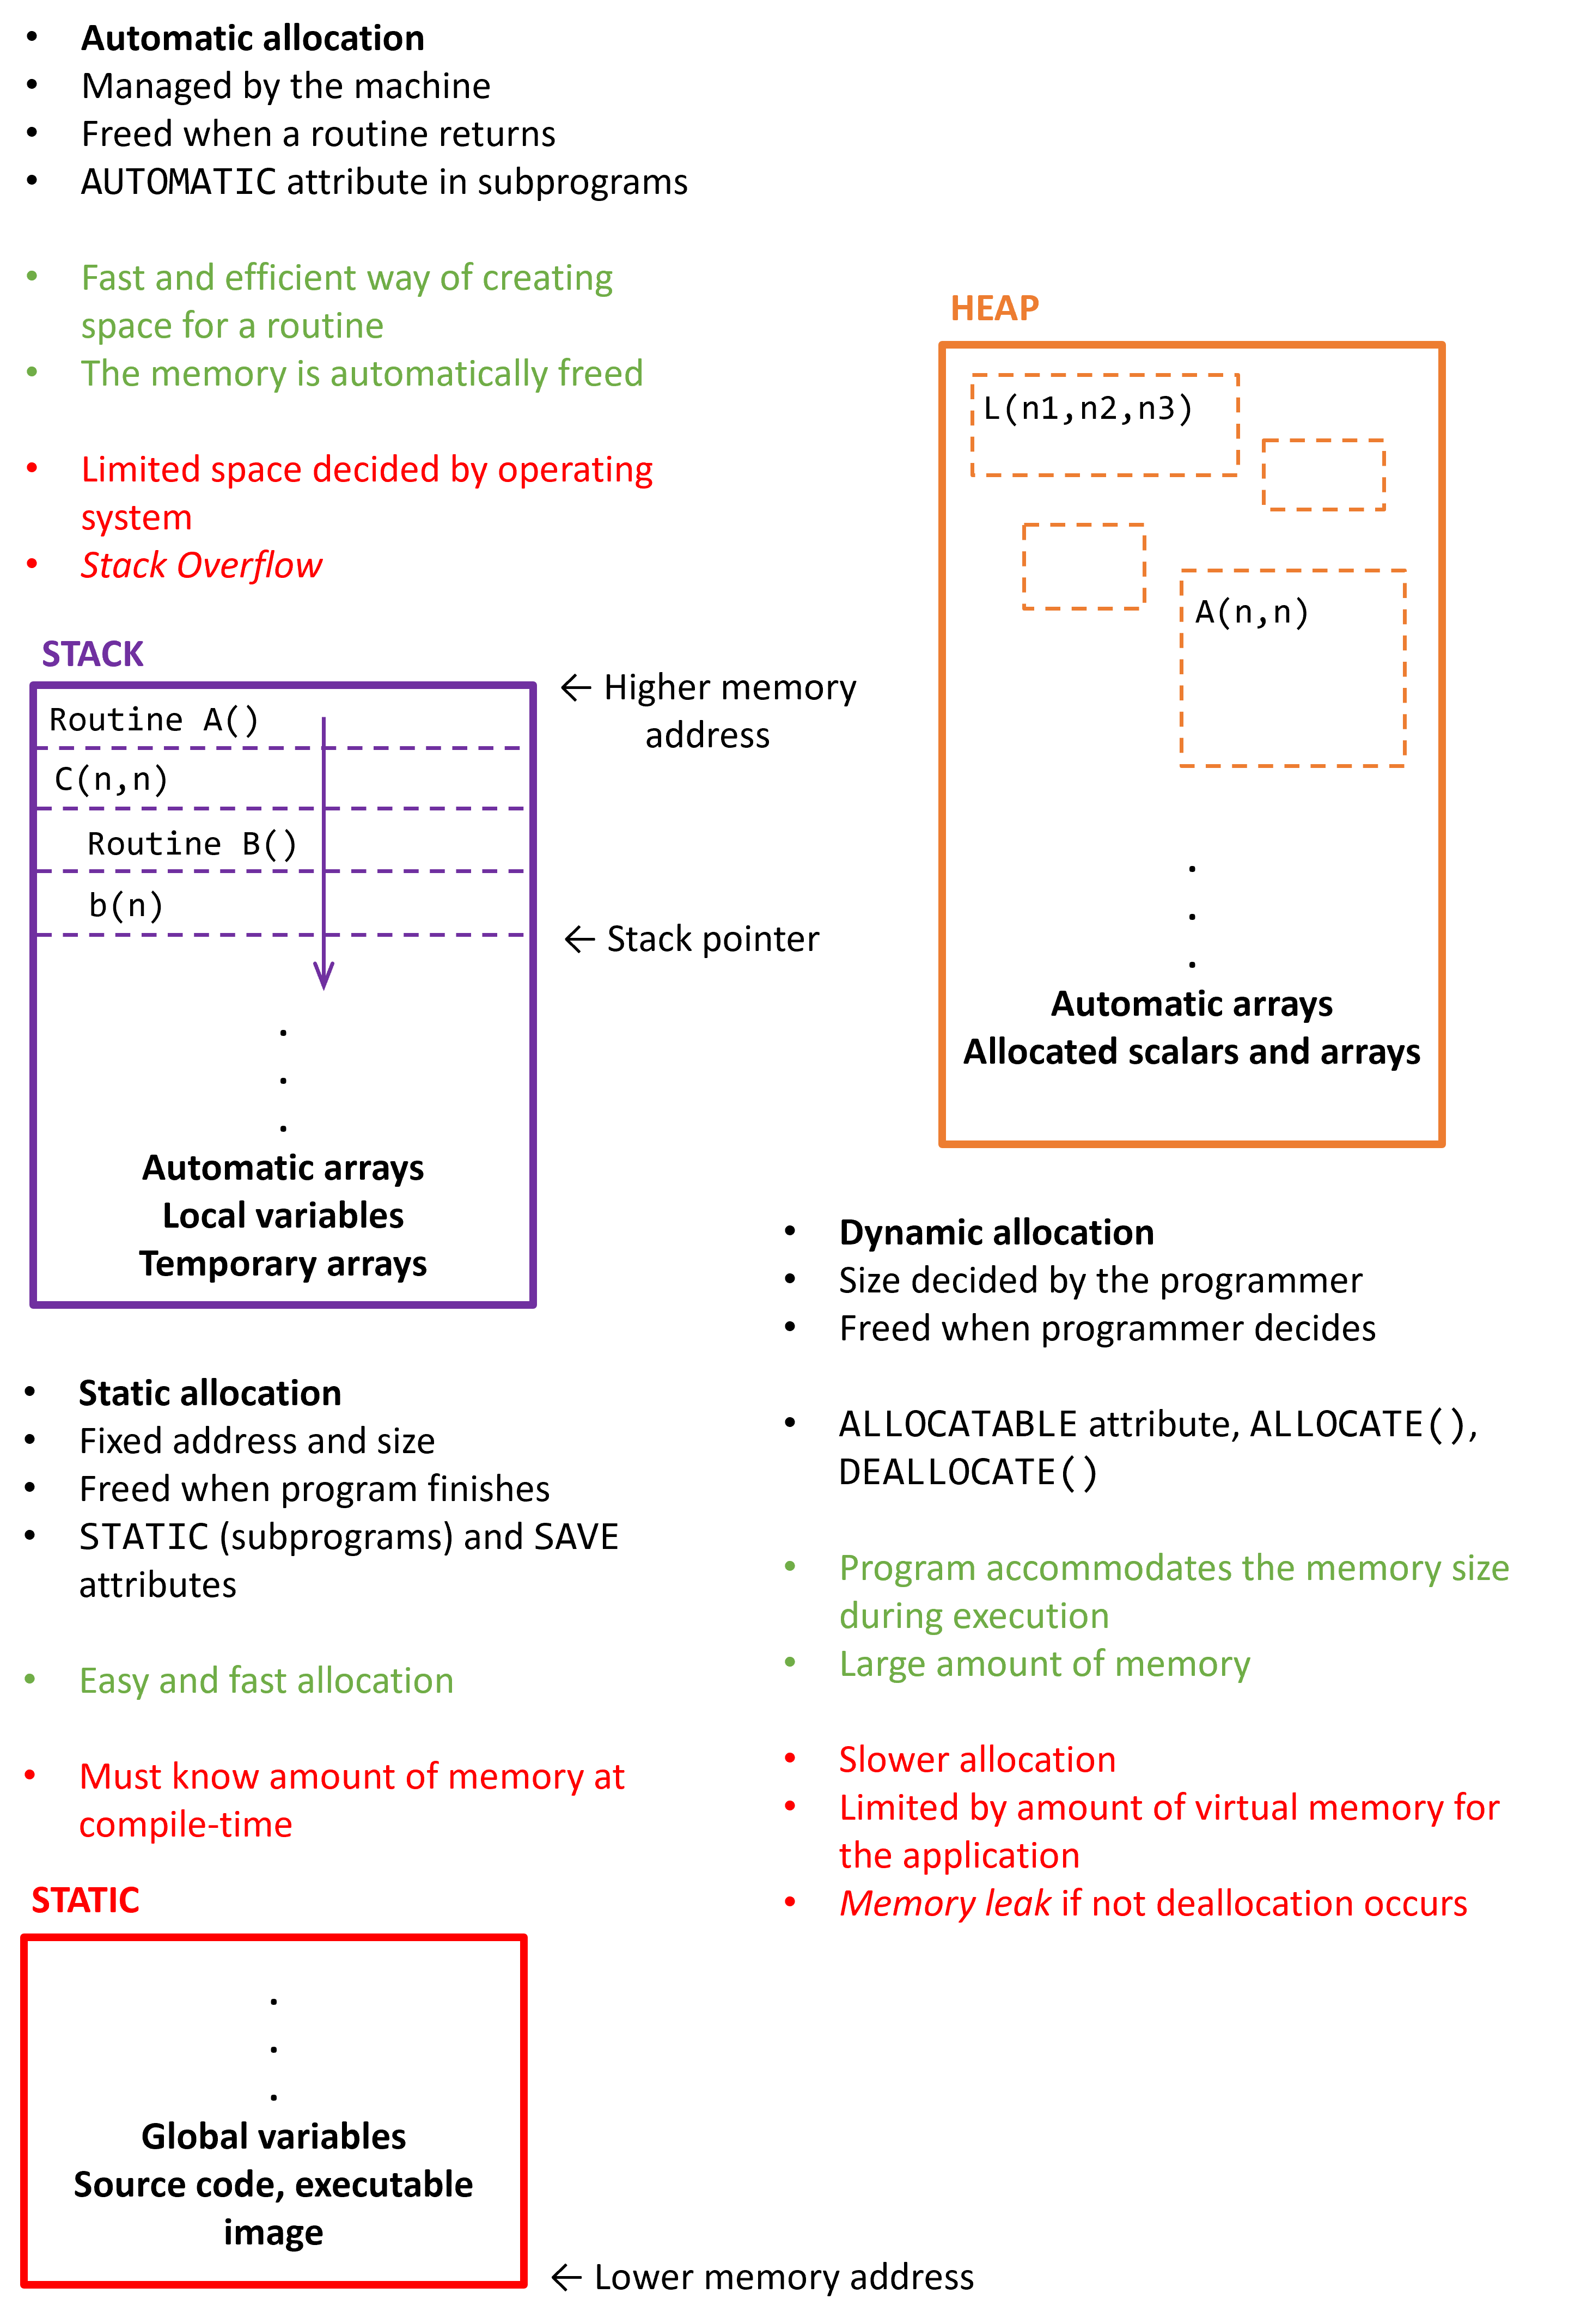
\includegraphics[width= \textwidth]{./doc/Figures/Memories.png}
    \caption{Three memory regions used by a program.}
    \label{fig:Memories}
\end{figure}

Let's revise some properties, advantages and problems associated to these memories:

\begin{itemize}
    \item \textbf{Static:} it is usually located in the low end of the memory reserved for the application. The compiler creates a list of variables to be allocated during compilation and gives them a fixed address 
    so the whole program can use these variables at any time and faster. 
    
    This static allocation requires knowing the amount of memory needed at compile-time.
    
    \item \textbf{Heap:} when a data object is allocated, the application requests an amount of memory to the system, if there is space available the system answers with the 
    starting address where storing the data. Once that memory is not needed any more, the program can ask the system to free that memory under the \texttt{deallocate} statement (in the case of Fortran) so
    that space becomes available for the next time. Notice that the amount of space for a program is bigger than the stack, but not unlimited, here concepts like virtual memory and swap play an important role. 
    
    For the heap a memory leak can happen if no deallocation is performed (the memory continue being used with not useful data) and it is normally slower than static allocation. 
    However, the programmer manages this space and the program decides how much memory to use for each purpose. 
    
    \item \textbf{Stack:} it is composed by a limited amount of memory and a pointer that holds the current position where routines can store local variables. This space is filled from the top to the bottom of the memory so any time that a subroutine or function (let's say \texttt{function A}) needs from temporary storage this space is used, the pointer is decremented and the stack space is reduced. If this function calls a nested \texttt{function B}, then its local variables are stored below variables of \texttt{A} and the pointer is decremented once again. Once the \texttt{routine B} finishes its operations, the pointer is incremented again below the spaced filled by \texttt{routine A} so that memory is available for the next routine. This structure is called LIFO; 'Last-In,-First-Out'.  
    
    The process is efficient and fast and the space is automatically freed when the routine returns to its host. This allocation is performed by the machine but the programmer usually has the option to declare some variables as \texttt{AUTOMATIC} in subprograms so they reside in the stack area. On the contrary, the amount of space is limited by the linker in the case of Windows and the programmer must be careful with allocating more space than it is available in order to avoid stack overflow. 
        
\end{itemize}


Stack overflow, when the memory allocated on the stack overflows into other memory regions, usually happens with two situations; extremely deep (or infinite) recursion and large array variables. 

%Primer ejemplo de stack overflow


The second example dynamically allocates a $400\times 400\times 400$ of 4-bytes reals array in the heap (\texttt{R})  but then the function \texttt{StackOverflow\_size( n )} tries to locate a similar automatic array (\texttt{S}) in the stack leading to a Stack Overflow error. 

\begin{verbatim}
real, allocatable :: R(:,:,:)
integer :: n

n = 400
allocate( R(n, n, n) )

R = StackOverflow_size( n ) 
\end{verbatim}

with the function:

\begin{verbatim}
function StackOverflow_size( n ) result(R)
integer, intent(in) :: n
real :: R(n, n, n)    

    R(:, :, :) = 1.

end function
\end{verbatim}

Some strategies can be used to avoid this error:

\begin{enumerate}
    \item Try to reduce the abuse of stack; allocate automatic arrays that usually goes to stack so they are located in heap. Then, they are automatically deallocated at the end of the routine. 
    
    \item The size of the Stack memory can be increased through a linker option. In Visual Studio for example it can be written: \texttt{/STACK:100000000} specifying the size in bytes desired.
    
    \item A compiler option can be used to change the default storing place for automatic arrays and temporary arrays so they are automatically located in the heap: \texttt{/heap-arrays}. If a kilobytes size is specified, only larger arrays are allocated to heap (i.e. \texttt{/heap-arrays100} to only affect arrays larger than 100 kilobytes). Use the value \texttt{0} to apply the behaviour to all arrays.  
    
\end{enumerate}


Now try to execute the second example with the option \texttt{/heap-arrays0} specified in the compilation options. For the case of Visual Studio it can be done in the project properties by clicking on Configuration Properties/Fortran/Command Line and adding that line.


%-------------------------------------------------------------------------------------------------------------
%MAYBE INTERESTING IN FUTURE:

%When using AUTOMATIC, SAVE, STATIC, etc.
%\item How to manage it in your program and recommendations.
%\item How to reserve more space in each of them.




%-------------------------------------------------------------------------------------------------------------
%Revise the following concepts:
%
%\begin{enumerate}
%    \item Who manages the memory.
%    \item Where are physically stored (RAM, swap).
%    \item Which is faster to allocate and use.
%    \item Common problems related to the use of that memory.
%    \item How to manage it in your program and recommendations.
%    \item How to reserve more space in each of them.
%    \item etc.
%\end{enumerate}


%  Fortran for example uses this memory to create space for local arrays (those based on arguments of routines) or for temporary copies in array expressions. 
%     the stack is managed by the CPU, there is no ability to modify it
% variables are allocated and freed automatically
%  
  